\section{非约态概形}

我们现在离开那些能被看作概形的对象,即那些仿射概形$\spec R$而$R$是有一个有限生成代数闭域上的代数,且没有幂零元。这里的现象将变得不再那么熟悉,我们需要在它们身上花费更多努力。

这类概形在一些足够简单的几何背景下就已经出现了:比如,下面处理的多重点已经作为两个寻常概形的相交或者作为映射“退化的”纤维出现了,正如Exercise \ref{exe.2.2}中看到的。另一类非约态概形重要的应用在一族簇的理论(theory of families of varieties):形变理论(deformation theory)以及模理论(moduli theory)。我们将解释如何对一族单参数的簇取极限,以及引入平坦性这一关键概念。最后,我们将给出一些非约态概形的例子,这些例子就它们自身而言都是有趣的对象。

从最简单的情况入手,我们将关注仿射空间$\mathbb{A}_K^n$的子概形,其支撑于原点\footnote{译者注:即其支撑只有这点。} ------ 等价地,它由一个理想$I$给出,其零点集$V(I)$作为集合只包含$(0$, $\dots$, $0)$. (回忆一个概形的支撑是指它自有的那个拓扑空间。)

\subsection{双重点}\label{s.2.3.1}
\index{双重!点}
\begin{exa}
	此类概形最简单的例子是$\mathbb{A}_K^1$由理想$(x^2)$定义的子概形 ------ 即概形$\spec K[x]/(x^2)$,通过商映射$K[x]\to K[x]/(x^2)$诱导的映射看作$\mathbb{A}_K^1$的子概形。这个概形只有一个点,对应于理想$(x)$,但同样作为$\mathbb{A}_K^1$的子概形与作为抽象概形,这与概形$\spec K[x]/(x)=\spec K$不同。作为抽象概形,我们能看到存在如下差别,在$X$上存在非零正则函数(比如$x$)在$X$唯一一点处为零,当然任意这样的函数平方为零。差别在于,作为$\mathbb{A}_K^1$的子概形,$\mathbb{A}_K^1$上的函数$f\in K[x]$在$X$上为零当且仅当$f$和它的一阶导数同时在点$0$为零。于是$X$上的函数包含两个数据,$\mathbb{A}_K^1$上的一个函数与它的一阶导数在点$0$的值。因为这个原因,有时我们将$X$叫做$\mathbb{A}_K^1$中点$0$的\textit{一阶邻域}\index{一阶!邻域}。
\end{exa}

更一般的,对于任意的$n$,理想$(x^n)$定义了一个子概形$X\subset \mathbb{A}_K^1$,它的坐标环为$K[x]/(x^n)$,$\mathbb{A}_K^1$上的函数$f(x)$在$X$上为零当且仅当$f$以及它的前$n-1$阶导数全都在点$0$处为零。

\begin{exa}[双重点]
理解双重点的下一步是考虑$\mathbb{A}_K^2=\spec K[x,y]$中支撑于原点的子概形,这个子概形需要同构于Example {{\addtocounter{thm}{-1}}\thethm{\addtocounter{thm}{1}}}中的那个子概形$X$. 令$Y\subset \mathbb{A}_K^2$是这样的一个子概形,$R=\mathscr{O}_Y(Y)\cong K[\varepsilon]/(\varepsilon^2)$是它的坐标环,以及满射
\[
	\varphi:K[x,y]\to R
\]
定义了$Y$到$\mathbb{A}_K^2$的含入。$R$中唯一的极大理想$\mm$在$K[x,y]$中的原像是对应于原点的理想$(x,y)$,因为在$R$中$\mm^2=0$,所以映射$\varphi$在$(x,y)^2=(x^2,xy,y^2)$上为零,于是诱导了映射
\[
	\bar\varphi:K[x,y]/(x^2,xy,y^2)\to R.
\]
等价地,$Y$必须包含在子概形
\[
	\spec K[x,y]/(x^2,xy,y^2)
\]
中。但环$K[x,y]/(x^2,xy,y^2)$是一个$K$上的三维矢量空间,$R$只有二维。这是因为,$\varphi$的核将包含一个非零齐次线性型$\alpha x+\beta y$,其中$\alpha$, $\beta\in K$. 记
\[
	X_{\alpha,\beta}=\spec K[x,y]/(x^2,xy,y^2,\alpha x+\beta y)\hookrightarrow \mathbb{A}_K^2.
\]
子概形$X_{\alpha,\beta}$能被下面的条件所刻画:

\begin{compactenum}[(i)]
\item 关联于函数$f\in K[x,y]$的理想的$\mathbb{A}^2_K$的子概形,在原点为零以及在那儿其偏导数满足
\[
	\beta\frac{\partial f}{\partial x}-\alpha\frac{\partial f}{\partial y}=0
\]
(因为这可以推出$f=c(\alpha x+\beta y)+\text{高阶项}$),或者
\item Example {{\addtocounter{thm}{-1}}\thethm{\addtocounter{thm}{1}}}中的子概形$X\subset \mathbb{A}_K^1$在$\mathbb{A}_K^1$到$\mathbb{A}_K^2$的含入映射下的像由$x\mapsto (\beta x,-\alpha x)$给出。
\end{compactenum}

经典语言下,子概形$X_{\alpha,\beta}$被称作包含点$(0,0)$以及一个在$\alpha x+\beta y=0$方向上“无穷接近的点”,我们下面在传统图像中以一个小箭头画出$X_{\alpha,\beta}$:

% \pic{6.png}

\noindent 这是打算用一个切空间的可区分的一维子空间在平面上来表示这个点(尽管箭头给出了印象,实际上没有可区分的切矢量)。\nottran
\end{exa}

% \begin{wrapfigure}{i}{140pt}\includegraphics[scale=0.5]{chap_2/pics/7.png}\end{wrapfigure}
在实践中,概形$X_{\alpha,\beta}$会怎么出现呢?一种方式是曲线的相交。比如,当我们想要处理一条直线$L$与一条圆锥曲线$C$相切,显然,只在集合论意义上处理它们的相交是不令人满意的:
一条直线与一条圆锥曲线应该相交两次。甚至,说$C\cap L$的交点“重数为二”也不是完全令人满意的:比如,交点应该决定直线$L$,正如在非相切的例子中那般。真正令人满意的定义是,$C\cap L$是由理想$I_C$与理想$I_L$的和决定的$\mathbb{A}_K^2$的子概形,使得,比如,直线$y=0$以及抛物线$y=x^2$将相交于子概形$X_{0,1}=\spec K[x,y](x^2,y)$. 作为平面中唯一包含于$X_{0,1}$的直线,这将完全决定$L$. 

另一个出现形如$X_{\alpha,\beta}$的子概形的重要方式是作为可约概形的极限。比如,考虑平面上一对不同的点$(0,0)$与$(a,b)$,它们的并是闭子概形
\[
	X=\{(0,0),(a,b)\}=\spec S\subset \mathbb{A}_K^2,
\]
其中
\[
\begin{aligned}
	S&=K[x,y]/\left((x,y)\cap (x-a,y-b)\right)\\
	&=K[x,y]/(x^2-ax,xy-bx,xy-ay,y^2-by).
\end{aligned}
\]
由中国剩余定理,$S\cong K\times K$. 于是,特别地,$S$(作为矢量空间)是一个二维$K$-代数。

现在假设点$(a,b)$沿着一条曲线$(a(t),b(t))$往$(0,0)$移动,其中$(a(0),b(0))=(0,0)$而$a$, $b$是$t$的多项式,我们记作
\[
	a(t)=a_1t+a_2t^2+\dots,\quad b(t)=b_1t+b_2t^2+\dots.
\]

% \begin{center}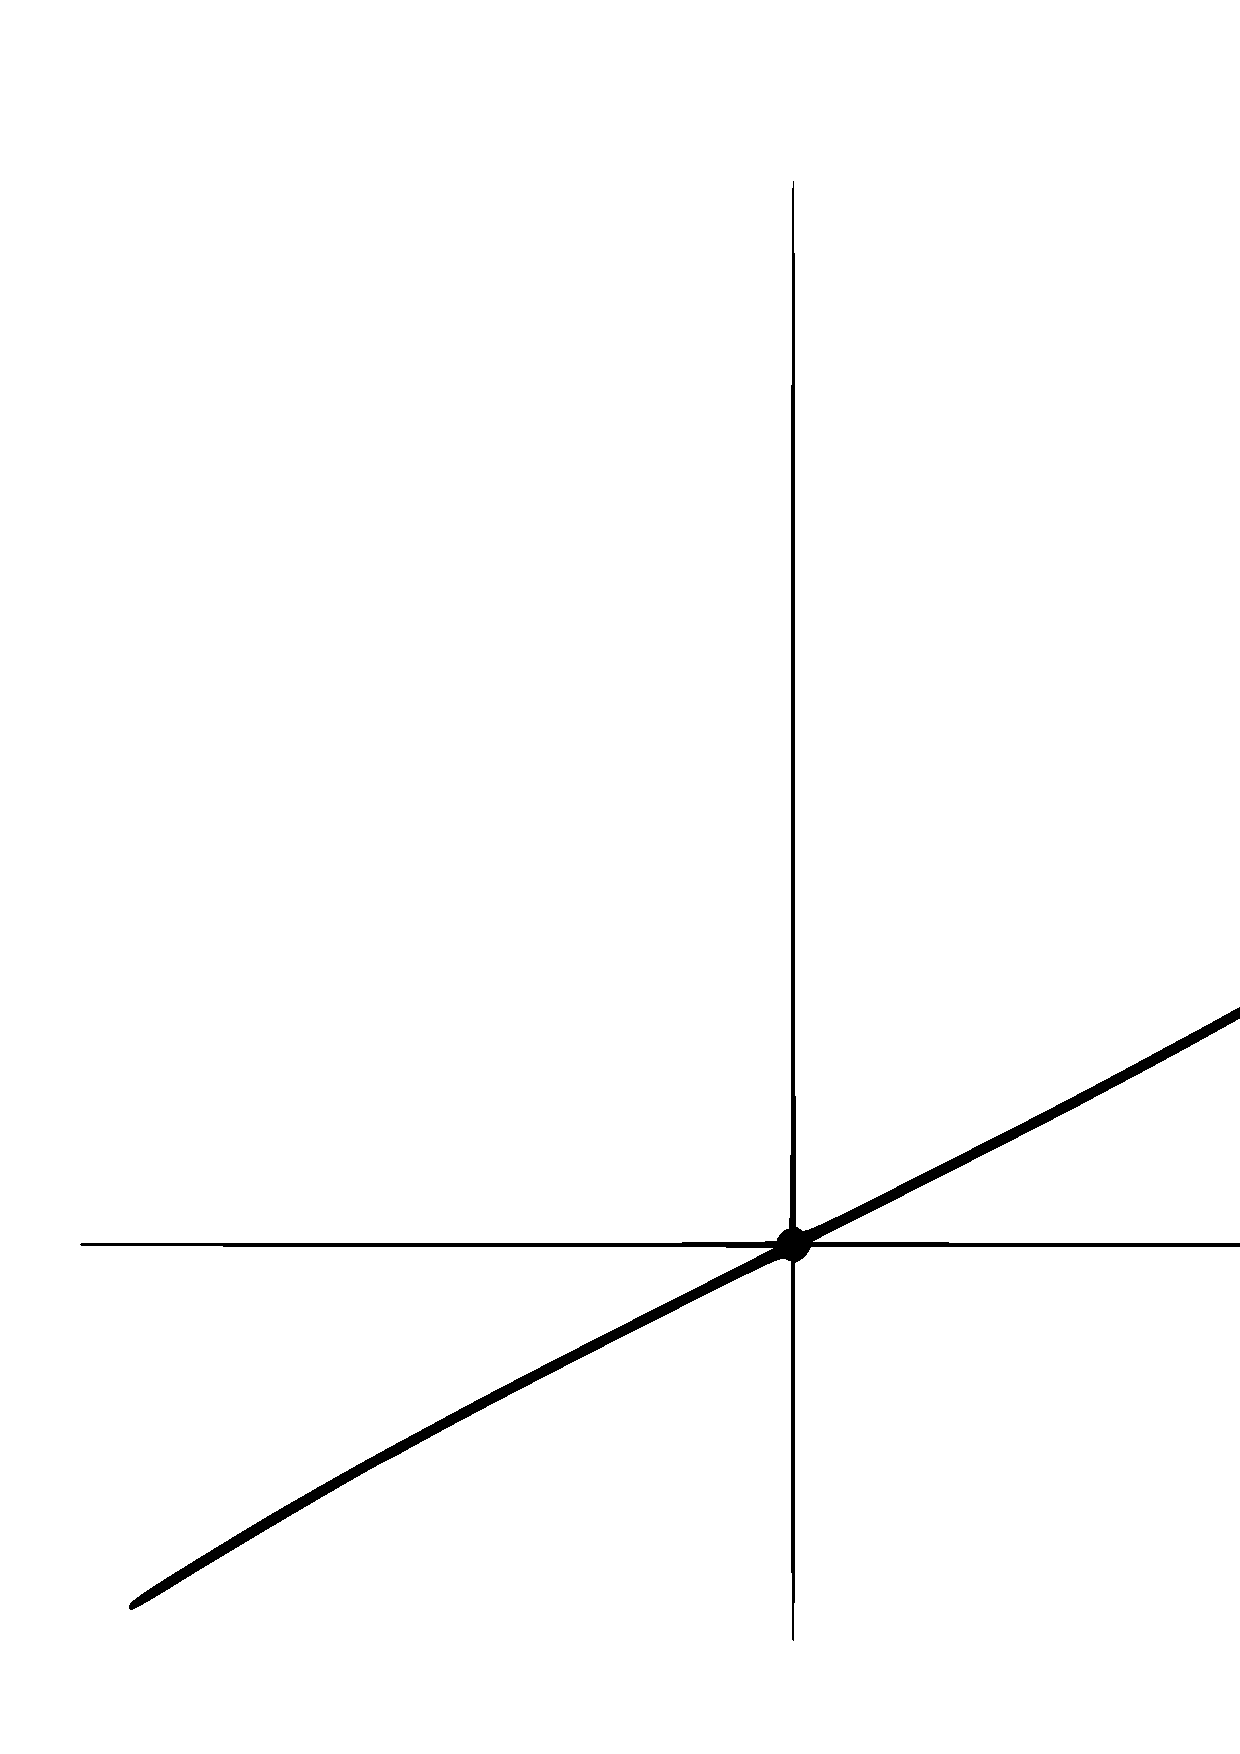
\includegraphics[scale=0.5]{chap_2/pics/8.png}\end{center}

那么$X_t=\{(0,0),(a(t),b(t))\}$在$t\to 0$的极限是什么呢?使用概形,我们能采用一种不常见的观点,在如下的合适表述下,此时它的极限依然是两个点:它将是一个仿射概形$X$,其坐标环依然是一个$K$上的二维矢量空间。我们可以取下面这族理想在$t\to 0$下的极限
\[
	I_t=(x,y)\cap (x-a(t),y-b(t)).
\]
作为关联于$X$的理想来定义$X$. 当然,这仅仅把困难转移到了描述什么是理想族的极限上!但这是简单的:在这个例子中,比如,我们能把它们的极限取为$K[x,y]$
中(看作$K$上的矢量空间时)余维数为$2$的子空间。这个极限依然是一个理想因为乘法是连续的。在理想的余维数是无限时,一个更精巧的解释是必要的,我们将在遇到一维概形族的极限以及再一次在3.3.2节中的射影情况下讨论这个问题。\nottran

为了看看上面说的在实践中是什么意思,首先观察$I_t$生成元$x^2-a(t)x$, $xy-b(t)x$, $xy-a(t)y$以及$y^2-b(t)y$,它们当$t\to 0$的时候有清楚的极限$x^2$, $xy$, $xy$和$y^2$,于是这些多项式应该在$I$中。此外,观察$I_t$包含线性型
\[
	a(t)y-b(t)x=(xy-b(t)x)-(xy-a(t)y),
\]
因此对$t\neq 0$,同样多项式
\[
	\frac{a(t)y-b(t)x}{t}=a_1y-b_1x+t(\dots)
\]
% \begin{wrapfigure}{i}{160pt}\includegraphics[scale=0.5]{chap_2/pics/9.png}\end{wrapfigure}
也在$I$中。于是,理想$I$同样也包含它的极限$a_1y-b_1x$,于是我们有$I\supset (x^2,xy,y^2,a_1y-b_1x)$. 但是上式右侧作为$K[x,y]$的子空间的余维数已经是$2$了。于是$I=(x^2,xy,y^2,a_1y-b_1x)$,以及,相应地,
\[
	\lim_{t\to 0}(X_t)=X_{\alpha,\beta},
\]
其中$\alpha=b_1$以及$\beta=-a_1$.

从这个例子我们看到,$X$作为$\mathbb{A}_K^2$的子概形,“记住”了$(a(t),b(t))$趋向$(0,0)$的方向:我们认为它包含原点以及原点处沿着直线$a_1y-b_1x=0$的切方向。这条直线是连接$(0,0)$以及$(a(t),b(t))$的直线$L_t$的极限,这就是说,这是曲线被参数化为$(a(t),b(t))$后在原点处的切线,正如图所示。

我们将在\ref{s.2.3.4}节看到如何推广极限的概念。

\subsection{多重点}

上一个例子中的子概形$X_{\alpha,\beta}$被称为平面上的“双重点”,这里\textit{双重}\index{双重!点}指坐标环
\[
	R=K[x,y]/(x^2,xy,y^2,\alpha x+\beta y)\cong K[t]/(t^2)
\]
作为$K$-模的矢量空间维数。一般地,如果$X=\spec R$是一个仿射概形,以及$R$是一个$K$上的有限维矢量空间%\footnote{译者注:即所谓的有限$K$-代数。}
,我们定义$X$相对于$K$的\idx{度}\label{deg}(degree)为$R$作为$K$-矢量空间的维度,记作$\deg_K(X)$或者再简单些$\deg(X)$. (当对域$K$不会产生歧义的时候,我们将在记号和行文中去掉脚标$K$.) 在这种情况下,我们称$\spec R$是一个\textit{有限$K$-概形}。\index{有限!概形}

下面考虑度为3及以上的例子。一些东西在这里将变得不一样了。首先,代数闭域$K$上的所有双重点 ------ 即仿射概形$\spec R$,其中$R$是一个维度为2的局部$K$-代数 ------ 是同构的,因为这样的$R$必然同构于$K[x]/(x^2)$. (证明:令$\mm$是$R$的极大理想,因为$K$没有有限维扩张,于是$R/\mm\cong K$. 因为$R$是二维的,$\mm$是一维的,所以$\mm^2=0$(比如,从Nakayama引理可以得到这点%\footnote{译者注:因为$\mm^2$作为$\mm$的子模,要么是一维的要么是$0$,如果是一维的,则$\mm=\mm^2$,此时由Nakayama引理,存在一个$a\in \mm$使得$am=m$对所有的$m\in \mm$都成立。注意到$\mm$是唯一的极大理想,所以$1-a$可逆,故$m=0$,这与$\mm$是一维的矛盾。}
)。于是从$K[x]$到$R$的自然满射的核包含$x^2$,这样$R$与$K[x]/(x^2)$的同构就已经给出了。)作为对比,对于三重点(度为3的点)这点并不正确:很轻松就可以看出概形
\[
	\spec K[x]/(x^3)\quad\text{和}\quad \spec K[x,y]/(x^2,xy,y^2)
\]
是不同构的。然而,任意三重点同构于上面两者中的一个,这个事实的证明我们留作下面的习题。

\begin{exe}
	设$K$是一个代数闭域,而$K=\spec K[x_1,$ $\dots$, $x_n]/I\subset \mathbb{A}_K^n$是任意的度为3的支撑于原点的零维子概形。证明,$Z$同构于$X=\spec K[x]/(x^3)$或者
	\[
		Y=\spec K[x,y]/(x^2,xy,y^2),
	\]
	以及$X$与$Y$并不同构。
\end{exe}

特别地,任意的$K$-矢量空间维度为3的环$K[x_1,$ $\dots$, $x_n]/I$能被两个$x_i$的线性型生成。几何上来看,这就是说,$\mathbb{A}_K^n$中度为3的点是平面的,即,处于一个线性子空间$\mathbb{A}_K^2\subset \mathbb{A}_K^n$上。在$\mathbb{A}_K^2$中,以上两类三重点能被实现为三个不同的点的极限。同构于$X$的那一类,能被看作三个点都来自于同一条非奇异曲线,然而同构于$Y$的那一类来自于当两个点以两个不同的方向趋向于第三个点。下面的练习包含了这个现象的例子。

\begin{exe}
	\begin{compactenum}[(i)]
		\item 证明,$\mathbb{A}_K^2$的由理想$(y-x^2,xy)$给出的子概形来自于在圆锥曲线$y=x^2$三个点的极限,这个子概形同构于上面的$X$,但是不包含$\mathbb{A}_K^2$的任意直线。

		% \pic{10.png}

		\item 证明,来自于当两个点以两个不同的方向趋向于第三个点极限的$\mathbb{A}_K^2$的子概形同构于上面的$Y$.
	\end{compactenum}
\end{exe}

\begin{exe} (对那些熟悉Grassmannian的人。)上面的例子可能让人觉得同构于$X$的概形是那些同构于$Y$的概形的极限。然而事实并不如人所愿,下面的例子与其刚好相反。令$\mathscr{H}$是$\mathbb{A}_K^2$中支撑于原点的度为$3$的有限子概形,$\mathscr{H}$可以通过六维矢量空间$K[x,y]/(x,y)^3$ 余维数为$3$的子空间们的Grassmannian的一个闭子概形自然地参数化。证明$\mathscr{H}$是一个曲面,其中一点对应于唯一的子概形$\spec K[x,y]/(x^2,xy,y^2)$,它同构于$Y$,其余的点对应于同构于$X$的子概形。证明,概形$\mathscr{H}$同构于$\mathbb{P}^3_K$中的一个二维立体圆锥,其顶点对应于$Y$.
\end{exe}

\begin{exe}
	令$C$是$\mathbb{A}_K^n$的由理想
	\[
	J=(x_2-x_1^2\text{, }x_3-x_1^3\text{, }\dots)
	\]
	给出的子概形。$C$中的一个闭点具有形式$f(t)=(t$, $t^2$, $t^3$, $\dots$, $t^n)$,其中$t\in K$,它有理想$(x_1-t$, $x_2-t^2$, $\dots)$. 考虑对$t\neq 0$的三点子概形
	\[
	X_t=\{f(0)\text{, }f(t)\text{, }f(2t)\}\subset C.
	\]

	\begin{compactenum}[(a)]
		\item 证明,当$t\to 0$时候概形$X_t$的极限是
		\[
		X_0=\spec K[x_1\text{, }\dots\text{, }x_n]/(x_2-x_1^2\text{, }x_1x_2\text{, }x_3\text{, }x_4\text{, }\dots\text{, }x_n),
		\]
		它同构于上面提到的三重点$\spec K[x]/(x^3)$.
		\item 证明,然而,$X_0$并不包含于$C$在原点的切线。而是,$X_0$包含的$\mathbb{A}_K^n$的最小线性子空间是$C$的密切平面
		\[
		x_3=x_4=\cdots=x_n=0,
		\]
		(回忆,按定义,这是切线以及$C$上原点附近其他点张成的平面在这些点趋向原点时的极限)\nottran,然而$C$的切线是$\mathbb{A}_K^n$的最小线性子空间包含$X_0$坐标环的极大理想的平方定义的子概形。于是,在这层意味上,$X_0$同时“记住”了$C$的切线与密切平面。
	\end{compactenum}
\end{exe}

\begin{exe}
	考虑对$t\neq 0$,子概形
	\[
	X_t=\{(0,0)\text{, }(t,0)\text{, }(0,t)\}\subset \mathbb{A}_K^2
	\]
	每个都包含了$\mathbb{A}_{K}^2$中三个不同的点。

	\begin{compactenum}[(a)]
		\item 证明,这族概形当$t\to 0$时的极限为
		\[
		X_0=\spec K[x,y]/(x^2,xy,y^2).
		\]
		\item 证明,$\mathbb{A}_K^2$上的函数$f\in K[x,y]$限制在$X_0$上决定了也被决定于它在原点的值以及在原点处任意方向的一阶导数值。于是我们可以认为$X_0$是$(0,0)$的一阶无穷小邻域。
		\item 证明,$X_0$包含于任意两条穿过$(0,0)$不同的直线的并中。
		\item 证明,$X_0$不包含于任意的非奇异曲线中,因此特别地,不是$\mathbb{A}_K^2$中任意两条非奇异曲线概形意义上的交。
	\end{compactenum}
\end{exe}

正如我们说的,两类三重点都可以嵌入到任意仿射空间中的平面中。但是四重点$\spec K[x$, $y$, $z]/(x,y,z)^2$不能,因为它的极大理想不能被两个元素所生成。其他新的现象将在空间(即不能包含在平面中)以及更高维度空间中的多重点上出现。比如,在四维仿射空间中不是每个度为$21$的点都可以写成$21$个不同的点的极限,就像下一个习题中所表现的那样。(同样可见Iarrobino [1985].)

\begin{exe}
	考虑$\mathbb{A}_K^4$的度为$21$零维子概形$\Gamma$,使得
	\[
	V(\mm^3)\subset \Gamma \subset V(\mm^4),
	\]
	其中$\mm$是$\mathbb{A}_K^4$中原点的极大理想。证明存在一个这样子概形的$84$维族,然后推出一个一般的这样的子概形不是一个约态概形的极限。
\end{exe}

\begin{exe}
	将$\mathbb{A}_K^2$的度为4和5的且支撑于原点的零维子概形分类到同构。其中哪些同构于$\spec K$上的概形。
\end{exe}

\begin{exe}
	一个支撑于一点的概形被称为\textit{曲线的},如果(局部)环的极大理想被一个元素生成,或者等价地,如果它的Zariski切空间的维度为0或者1. (这个名字来自于如下事实:正好就是这些概形能被包含于一条非奇异曲线中。)证明,对任意两个度为2且支撑于一点的$\mathbb{A}_K^2$的子概形,可以通过一个平面的线性变换从一个变成另一个,但是对长为3的曲线概形就不对了。(但注意,任意有着相同的度的两个$\mathbb{A}_K^2$的曲线子概形\textit{能}通过一个$\mathbb{A}_K^2$的自同构从一个变到另一个。)
\end{exe}

\begin{exe}
	(对那些熟悉曲线的人。)对度为7的支撑于原点的3维仿射空间的子概形,存在无限多的同构型。对度为8的支撑于原点的仿射平面的子概形,存在无限多的同构型。
\end{exe}

正如所预料的那样,非代数闭域上非约态概形的行为将变得更加复杂。下面的习题给给出一个例子。

\begin{exe}
	分类所有度为2和3的$\rr$上支撑于$\mathbb{A}_\rr^2$原点的概形。$\rr$上的概形$X$的复化指$\cc$上的概形$X\times_{\spec \rr}\spec \cc$. 特别地,证明尽管$\rr$上每个复化同构于$\spec \cc[x]/(x^3)$的概形都同构于$\spec \rr[x]/(x^3)$,但存在且只存在两个不同构概形$X$,它们的复化都同构于$\spec \cc[x,y]/(x^2,xy,y^2)$.
\end{exe}

\subsubsection*{度与重数}
\addcontentsline{toc}{subsubsection}{度与重数}

回忆在第\pageref{deg}页,我们定义了一个有限仿射$K$-概形$X=\spec R$的\textit{度}是$R$作为$K$-矢量空间的维度,其中$R$是有限维的。当$K$是代数闭的时候,这样一个概形$X$的度,从某种角度来说,度量了它的非约态的程度。然而,就像最后一个习题所展现的,在一般的情况下这并不是正确的:$\spec \cc$是约态的,但是作为$R$上的概形,它的度为2.

这里有另一个概念,称为重数(multiplicity),它度量了$X$非约态的程度。与度依赖于基域$K\subset R$选取不同,重数是$X$本身的不变量,它在更一般的情况下有定义 ------ 我们这里将在任意Krull维数为零局部环$R$(即任意Artin局部环)上定义它。

令$R$是任意的零维局部环,它的极大理想是$\mm$. 可以选取$R$的一列理想
\[
	R\supset \mm = I_1\supset I_2\supset \cdots \supset I_{l-1}\supset I_l=0
\]
使得每一个商$I_j/I_{j+1}$作为$R$-模同构于$R/\mm$. (比如,我们能从一个比较粗的列
\[
	R\supset \mm \supset \mm^2\supset \cdots \supset 0
\]
开始,然后不断选取任意$R/\mm$-矢量空间$\mm^j/\mm^{j+1}$的子空间来加细它。)尽管这样一条列不唯一,但是它的长度$l$确实与选取无关的,我们定义$l$为环$R$或者零维概形$X$的\textit{重数}或者\textit{长度}\index{长度!环的}\index{长度!概形的}(比如见Eisenbud [1995, Section 2.4])。注意在原来的情况,当$R$是一个$K$上的有限维矢量空间时,剩余类域$R/\mm=\kappa$是$K$的一个有限扩张,所以我们有关系
\[
	\deg_K(X)=[\kappa:K]~\mathrm{mult}(X).
\]

对于任意的零维概形$X$,以及点$p\in X$,我们定义$X$在点$p$处的\textit{重数}为局部环$\mathscr{O}_{X,p}$的重数,记作$\mathrm{mult}_p(X)$. 如果$X$是一个有限$K$-概形,则$X$相对于$K$的度由
\[
	\deg_K(X)=\sum_{p\in X}[\kappa(p):K]~\mathrm{mult}_p(X)
\]
给出。

在第三章,我们将看到度和重数的概念如何拓展到正维数的概形上面去。

\subsection{嵌入点}

我们现在考虑一些高维非约态概形的例子,为简单起见,我们只考虑基本的约态概形是一条直线。\nottran 尽管如此,大量可能的行为出现了,比如,存在概形除了一点外看起来都像约态概形,或者存在概形处处都是约态。在这一小节中,我们考虑前者。术语上,我们称概形$X=\spec K[x_1$, $\dots$, $x_n]/I\subset \bba_{K}^n$有一个嵌入组分,如果某个开集$U\subset \mathbb{A}^n_K$交$X$于一个$X$的稠密子集,且$X\cap U$(定义于\ref{s.1.2.1}小节)的闭包并不等于$X$;或者,等价地,理想$I$的准素分解包含嵌入素理想们(见下面对准素分解的讨论)。如果嵌入素理想是极大的(等价地,如果$U$可以取为一个点的补),我们谈论的是\textit{嵌入点},因为我们下面讨论的概形$X$都是一维的,这是我们会看到的。\nottran

除了在一点外都是约态的非约态概形最简单的例子是$X=\spec K[x,y]/(y^2,xy)\subset \bba_K^2$. 理想$I=(y^2,xy)\subset K[x,y]$是在直线$y=0$为零以及在点$(0,0)$有二阶零点的平面上的函数构成的理想。代数上来讲,这就意味着$(y^2,xy)=(y)\cap (x,y)^2$. 于是,我们可以将概形$X$看作直线$y=0$稍作变形得到的,即,$X$上的函数$f$被其在$y=0$上的限制$f(x,0)$与其在$(0,0)$处沿着直线的导数$\partial f/\partial y(0,0)$所定义。

将$X$具象为一条由$y=0$定义的直线与一个非约化点的并是比较方便的,比如,由理想$(x^2,xy,y^2)$定义的“原点的一阶邻域”。

% \pic{11.png}

这样的准素分解对任意概形是存在的:我们这里简单地回顾一下代数基础知识。更多的细节,比如可见,Eisenbud [1995]; Atiyah \& Macdonald [1969]或者是这些参考文献中可能最平易近人的,Northcott [1953].

\subsubsection*{准素分解}
\addcontentsline{toc}{subsubsection}{准素分解}

给定Noether环$R$中的一个理想$I$,我们定义关联于$I$的素理想是那些素理想$\pp$使得$\pp$是$R/I$中某个元素的零化子。这个素理想构成了一个有限集。

一个理想$\mathfrak{q}\subset \pp$被称为$\pp$-准素的,如果$\pp$是$\mathfrak{q}$的根(那些存在一个幂在$\mathfrak{q}$中的元素构成的集合),任取$f$, $g\in R$满足$fg\in \mathfrak{q}$但$f\not\in \pp$,则我们有$g\in\mathfrak{q}$;等价地,$\mathfrak{q}$是$\pp$-准素的,如果$\pp$是它的根以及局部化映射$R/\mathfrak{q}\to R_{\pp}/\mathfrak{q}R_\pp$是一个单射。

任意理想$I$能被表为一族准素理想的交。因为准素于某素理想的理想们相交依然准素于这个素理想,$I$甚至能被表为准素于不同素理想的理想的交。如果我们有了这样一个分解,使得每一个准素理想都准素于不同素理想,且在该分解中不能再去掉任意的准素理想,此时这样的分解就被称为$I$的一个\textit{准素分解},此分解中的准素理想就被称为\textit{准素组分}。

关联于$I$的素理想就是那些准素组分的根。给定一个关联于$I$的素理想$\pp$,$I$的$\pp$-准素组分不由$I$唯一决定,然而,如果当$\pp$在关联于$I$的素理想中是极小素理想时,$I$的$\pp$-准素组分由$I$唯一决定。这样的准素组分被称为\textit{孤立组分}。

\begin{exe}
	取$I=(y^2,xy)$,分解
	\[
	I=(y)\cap (x,y)^2
	\]
	已经将$I$分解为两个准素理想的交(第一个是素理想,第二个准素于$(x,y)$)。
\end{exe}

因为$(y)$或者$(x,y)^2$都不能从上述分解中略去,这是一个准素分解,与其关联的概形$X$(正如下面定义的)就是直线$X_{\mathrm{red}}$以及在原点处的约态点。关联于$(x,y)$的准素组分在分解中不是唯一的,它可以取作$(x,y^2)$或者$(x+y,y^2)$,或者实际上无数多这样的理想中的任意一个,以及它们的交$(x^2,xy,y^2)$,或者对任意的$n\geq 2$,理想$(x^2,xy,y^2)$. 当然,对应于$(y)$的准素组分$(y)$是唯一的,因为$X_{\mathrm{red}}$并不包含于其他任意的关联概形中。

尽管有这种不唯一性,但对关联于一个给定的素理想$\pp$的准素组分却有一个良定的\textit{长度}概念,不需要写出准素分解,它等于环$R_\pp/IR_\pp$中最长的有限长理想的长度。这里一个模$M$的长度是指子模链
\[
	M\supsetneqq M_1 \supsetneqq M_2 \supsetneqq \cdots \supsetneqq M_{l-1} \supsetneqq M_l=0
\]
的最长长度。

\begin{exe}
	$(xy,y^2)$在原点处的准素组分的长度是$1$.
\end{exe}

\subsection{概形的平坦族}\label{s.2.3.4}

概形族是一个相当一般的概形,我们仅将一族概形定义为一个概形间的态射$\pi:X\to B$!族中的概形是$\pi$在$B$上点的纤维。这个概念包含了其他我们能想到的概念,比如一个“含参方程”定义的概形,$B$这是是参数变动的空间。

然而,概形族仅定义为一个任意态射$\pi:X\to B$实在太过一般以至于几乎没啥用,因为这个概形族的纤维可能完全不同。比如,给出一族概形$\pi:X\to B$与一个$B$的闭点$b$,将$X$替换为$X-\pi^{-1}b$与一些其他概形$Y$的不交并,然后将所有$Y$都映射到$b$,我们就构造了一个新的概形族,此时$b$的纤维就变成了$Y$. 因此,如果想要概形族在某种合理的意义上连续地变化,我们必须加上其他条件。这里的“合理”意指什么并不是显然的。至少要求它包含所有的连续变化族的母亲是自然的,即给定度的射影平面曲线(见3.2.8节)。其他例子是由多项式环中有着常有限余维数的理想族定义的概形族,就像我们在多重点的极限那里考虑的那样。

在许多几何理论中,我们能通过要求该族局部平凡得到一个连续变化族的正确概念,即,在某种合适的意义上,这族局部看来像是一个直积往一个因子的投影\footnote{译者注:比如纤维丛。}。但这对我们来说有两点错误。首先,如果我们天真地尝试对概形做同样的事情,将局部理解为Zariski拓扑中的局部,我们将得到了一个限制太多而无用的概念。一个更世故的方法是将局部平凡性要求成解析的,就是说,对$x\in X$以及$b=\pi(x)$,要求局部环$\oo_{X,x}$的完备化看起来像一个局部环$\oo_{B,b}$的完备化上的幂级数环。这个概念非常有用(被称为\textit{光滑}),但是它排除了,比如,一族给定度的平面曲线,因为光滑族不能有奇异纤维。光滑性同样排除了上一节中处理的族,不同点的不交并趋向于一个多重点,在多重点处,上述判据不能被满足。因此,我们必须寻找一个更一般的概念。

这种一般概念的最佳候选人是\textit{平坦性}。为了了解这个定义的动机,我们首先考虑更直观的极限概念。

\subsubsection*{极限}
\addcontentsline{toc}{subsubsection}{极限}

理解平坦性的几何内含的起点是概形的单参数族的极限概念。

我们从比较具体的东西开始:$B$上的\textit{给定概形$A$的闭子概形族}是一个$B\times A$的闭子概形$X\subset B\times A$和限制在$X$上的投射映射$B\times A\to B$,于是$X$在点$b\in B$上的纤维自然是$B\times A$在$B$上的纤维$A_b$的闭子概形。

令$B$是一个非奇异一维概形,典型地,我们对$R=K[t]$, $K[t]_{(t)}$或者$K[\![t]\!]$考虑$\spec R$,尽管任意的Dedekind整环(包含$\zz$或者$\zz_{(p)}$)也行。令$0\in B$是任意的闭点,即$B^*=B\setminus \{0\}$是$B$关于$\{0\}$的补。令$\mathbb{A}_B^n$和$\bba_{B^*}^n$是一般意义上,$B$与$B^*$上的$n$维仿射空间。

考虑一个$\bba_{B^*}^n=\bba_\zz^n\times B^*$的闭子概形$\mathscr{X}^*$,我们可以将其看作一个由$B^*$参数化的闭仿射概形族,即,对每一个$b\in B^*$,令$X_b=\pi^{-1}(b)$是投影$\pi:\mathscr{X}^*\to \bba_{B^*}^n\to B^*$的纤维,以及将这些概形$X_b$看作一个族。(在$B=\spec R$,其中$R=K[t]$或者$K[t]_{(t)}$的情况中,我们能将$\mathscr{X}^*$看作“$\mathbb{A}_K^n$中随着参数$t$改变的子概形族”。)我们问这样一个基本的问题:概形$X_b$在$b$趋向于$0$时候的极限是什么?

% \pic{12.png}

答案,也是唯一可能的答案,足够简单:因为概形族$X_b$的极限在任何合理的意义下都必须纳入一个包含所有概形$X_b$的族中,我们取$\mathscr{X}\subset \mathbb{A}_B^n$为$\mathscr{X}^*$在$\bba_B^n$中的闭包$\overline{\mathscr{X}^*}$,以及取概形族的极限$\lim_{b\to 0}X_b$为$\mathscr{X}$在点$0\in B$处的纤维$X_0$.

更具体些,若$B=\spec R$是仿射概形,以及$t\in R$是对应于点$0\in B$的极大理想$\mm\subset R$的一个生成元(于是$B^*=\spec R[t^{-1}]$),以及$I(\mathscr{X}^*)\subset R[t^{-1}][x_1$, $\dots$, $x_n])$是$\mathscr{X}^*\subset \bba_{B^*}^n$的理想,于是子概形$\mathscr{X}\subset \bba_{B}^n$的理想是交
\[
	I(\mathscr{X})=I(\mathscr{X}^*)\cap R[x_1,\,\dots,\,x_n].
\]
为了再具体些,如果我们取$B=\spec K[t]$,在概形$X_t$上为零的多项式的极限上极限概形$X_0\subset \bba_K^n$为零\footnote{原文是``the limiting scheme $X_0\subset \bba_K^n$ is cut out by the limits of polynomials vanishing on the schemes $X_t$''.}\nottran ,换句话说,如果我们将理想$I(X_t)\subset K[x_1$, $\dots$, $x_n]$看作$K$-矢量空间$K[x_1$, $\dots$, $x_n]$的线性子空间,以及令$V\subset K[x_1$, $\dots$, $x_n]$是平面族$I(X_t)$的极限位置\nottran ,则理想$I(X_0)$被$V$所生成。于是,这个极限的定义扩展了第\ref{s.2.3.1}节中用过的朴素极限概念。

举个例子,取$B=\spec K[t]$以及$B^*=B\setminus \{0\}=\spec K[t,t^{-1}]$,以及令$\bba_K^1$的子概形$X_t$包含两个点,坐标分别为$t$和$-t$,即,取$\mathscr{X}^*=V(x^2-t^2)\subset \spec K[t,t^{-1}][x]=\bba_{B^*}^1$. 于是,在$\bba_B^n$中,$\mathscr{X}^*$的闭包$\mathscr{X}$同样被$X=V(x^2-t^2)\subset \spec K[t][x]=\mathbb{A}_B^1$给出,以及$\mathscr{X}$在点$0\in B$的纤维$X_0$就是双重点$X_0=V(x^2)\subset\bba_K^1$.

概形族$\mathscr{X}^*\subset \bba_{B^*}^n$的极限概念非常依赖于到$\bba_{B^*}^n$的嵌入,而不仅依赖抽象族$\mathscr{X}^*\to B^*$. 于是,在上面的例子中,概形族$\mathscr{Y}^*=V(x^2-1)$以及概形族$\mathscr{Z}^*=V(x^2-t^{-2})\subset \spec K[t,t^{-1}][x]=\bba_{B^*}^1$作为$B^*$-概形是同构的,但是$\mathscr{Y}^*$的极限是两个约态点$V(x^2-1)\subset \bba^1_K$而$\mathscr{Z}^*$的极限是空集。

\subsubsection*{例子}
\addcontentsline{toc}{subsubsection}{例子}

现在我们遇到的极限的例子都是零维度概形的极限。这里有一些涉及正维的例子。 它们也是有启发性的,因为它们说明了嵌入点如何在簇的极限中自然地出现。

\subsubsection*{平坦性}
\addcontentsline{toc}{subsubsection}{平坦性}

\begin{defi}
	设$R$是一个环而模$M$是$R$-模,如果对任意的$R$-模单同态$A\to B$,诱导的映射$M\otimes_R A\to M\otimes_R B$依然是单同态的,则称$M$是平坦的。
\end{defi}

特别地,任意的自由模都是平坦的,于是,如果$R$是一个域,则每一个模都是平坦的。如果$R$是一个Dedekind整环,不难证明,$M$是平坦的当且仅当$M$是无挠的。我们下面建立与之对应的几何定义:

\begin{defi}
	一族概形间的态射$\pi:X\to B$是平坦的,如果对每一个$x\in X$,局部环$\mathscr{O}_{X,x}$通过映射$\pi^\#$作为$\mathscr{O}_{B,\pi(x)}$-模时是平坦的。
\end{defi}

这个概念已足够一般到包含给定度的平面曲线族,但也足够限制,使得平坦族中概形有很多共同点。这是非常令人满意的,除了(最初,至少)它似乎不是一个非常“几何”的性质。 然而,这实际上是上面介绍的朴素极限概念的最自然的( 事实上,这是唯一可能的)拓展! 我们将建立这个事实,然后继续考虑其他平坦性的性质; 不错的技术讨论见Eisenbud [1995]; Matsumura [1986]; Hartshorne [1977]. \nottran

\begin{pro}
	令$B=\spec R$是一个非奇异一维仿射概形,$0\in B$是一个闭点以及$B^*=B\setminus \{0\}$. 令$\mathscr{X}\subset \bba_{B}^n$是任意的闭子概形,以及投影$\pi:\mathscr{X}\to B$. 下面的条件是等价的:
	\begin{compactenum}[\((1)\)]
		\item $\pi$在点$0$处平坦。
		\item 纤维$X_0=\pi^{-1}(0)$是纤维族$X_b=\pi^{-1}(b)$在$b\to 0$时的极限。
		\item $X$没有支撑于$X_0$的不可约组分或者嵌入组分。
	\end{compactenum}
\end{pro}

\begin{lem}
	令$K$是一个域,$B$是一个约态$K$-概形,$b\in B$是一个闭点,而$\mathscr{X}\subset \bba_{B}^n$是一个闭子概形。 $\mathscr{X}$在点$b$处平坦当且仅当,对每一个非奇异一维$K$-概形$B'$,每一个闭点$0\in B'$以及任意将$0$变成$b$的态射$\varphi:B'\to B$,纤维$X_b$是纤维$X_{\varphi(b')}$在$b'$趋向于$0$时候的极限,即,对任意将$0$变成$b$的态射$\varphi:B'\to B$,拉回族
	\[
	\mathscr{X}'=\mathscr{X}\times_B B'\subset \bba_{B'}^n\to B'
	\]
	在点$0$处平坦。
\end{lem}

\subsection{多重直线}

我们现在考虑一个非约态仿射概形$X$,它没有嵌入组分且支撑于一条直线。我们将假设这条直线的重数(准素分解意义上)是$2$. 下面我们分析各种可能性。

很容易写出第一个例子:概形
\[
	X=\spec K[x,y]/(y^2)\subset \bba_K^2
\]
显然有我们想要的性质。很清楚,在$\bba_K^2$中此外再无支撑于直线$y=0$的例子,不过我们能在$\bba_K^3$中构造不少。

% \pic{14.png}

\begin{exe}
如果$p$, $q$是互素的多项式,于是环
\[
	K[x,y,z]/I_{p,q}
\]
中的理想
\[
	(x,y)/I_{p,q}
\]
是秩为$1$的无挠$K[z]$-模,于是$X_{p,q}$是准素的,$(X_{p,q})_{\text{red}}$是直线$\spec K[x,y,z]/(x,y)$,以及$X_{p,q}$的重数为$2$.
\end{exe}

\begin{exe}
	证明,如果$A$一个Noether $K$-代数,使得$X=\spec A$没有嵌入组分,重数为$2$,以及满足$X_{\text{red}}\cong \bba_K^1$,于是$X$同构于$\spec K[x,y]/(y^2)$.
\end{exe}

我们将在下一章看到,这个例子与投射空间中的情况产生了对比:那里有许多不同构的投射双重直线。